\section*{Homework 2}

Given the system of equations, remove a set of 2 variables aside from $\left\{ x_1, x_4 \right\}$.

\begin{align*}
	x_1 + 2x_2 + 3x_3 &= 6 \\
	x_1 + x_2 + x_3 + x_4 &= 4 \\
	x_1, x_2, x_3, x_4 &\geq 0 \\
\end{align*}

For this homework we will remove $\left\{ x_2, x_4 \right\}$.

Step 1: Solve for $x_2$.

\begin{align*}
	x_1 + 2x_2 + 3x_3 &= 6 \\
	2x_2 &= 6 - 1x_1 - 3x_3 \\
	x_2 &= 3 - \frac{1}{2}x_1 - \frac{3}{2}x_3 
\end{align*}

Step 2: Solve for $x_4$. Plug in $x_2$.

\begin{align*}
	x_1 + x_2 + x_3 + x_4 &= 4 \\
	x_1 + 3 - \frac{1}{2}x_1 - \frac{3}{2}x_3 + x_3 + x_4 &= 4 \\
	3 + \frac{1}{2}x_1 - \frac{1}{2}x_3 + x_4 &= 4 \\
	x_4 &= 1 + \frac{1}{2}x_3 - \frac{1}{2}x_1
\end{align*}

Step 3: Handle non-negativity constraint. Simplify.

\begin{align*}
	3 - \frac{1}{2}x_1 - \frac{3}{2}x_3 &\geq 0 \\
	- \frac{1}{2}x_1 - \frac{3}{2}x_3 &\geq -3 \\
	\frac{1}{2}x_1 + \frac{3}{2}x_3 &\leq 3 \\
	x_1 + 3x_3 &\leq 6
\end{align*}

\begin{align*}
	1 + \frac{1}{2}x_3 - \frac{1}{2}x_1 &\geq 0 \\
	x_1 - x_3 &\leq 2
\end{align*}

So our new setup is:

\begin{align*}
	x_1 + 3x_3 &\leq 6 \\
	x_1 - x_3 &\leq 2 \\
	x_1, x_3 &\geq 0
\end{align*}

\begin{figure}[htbp]
    \centering
    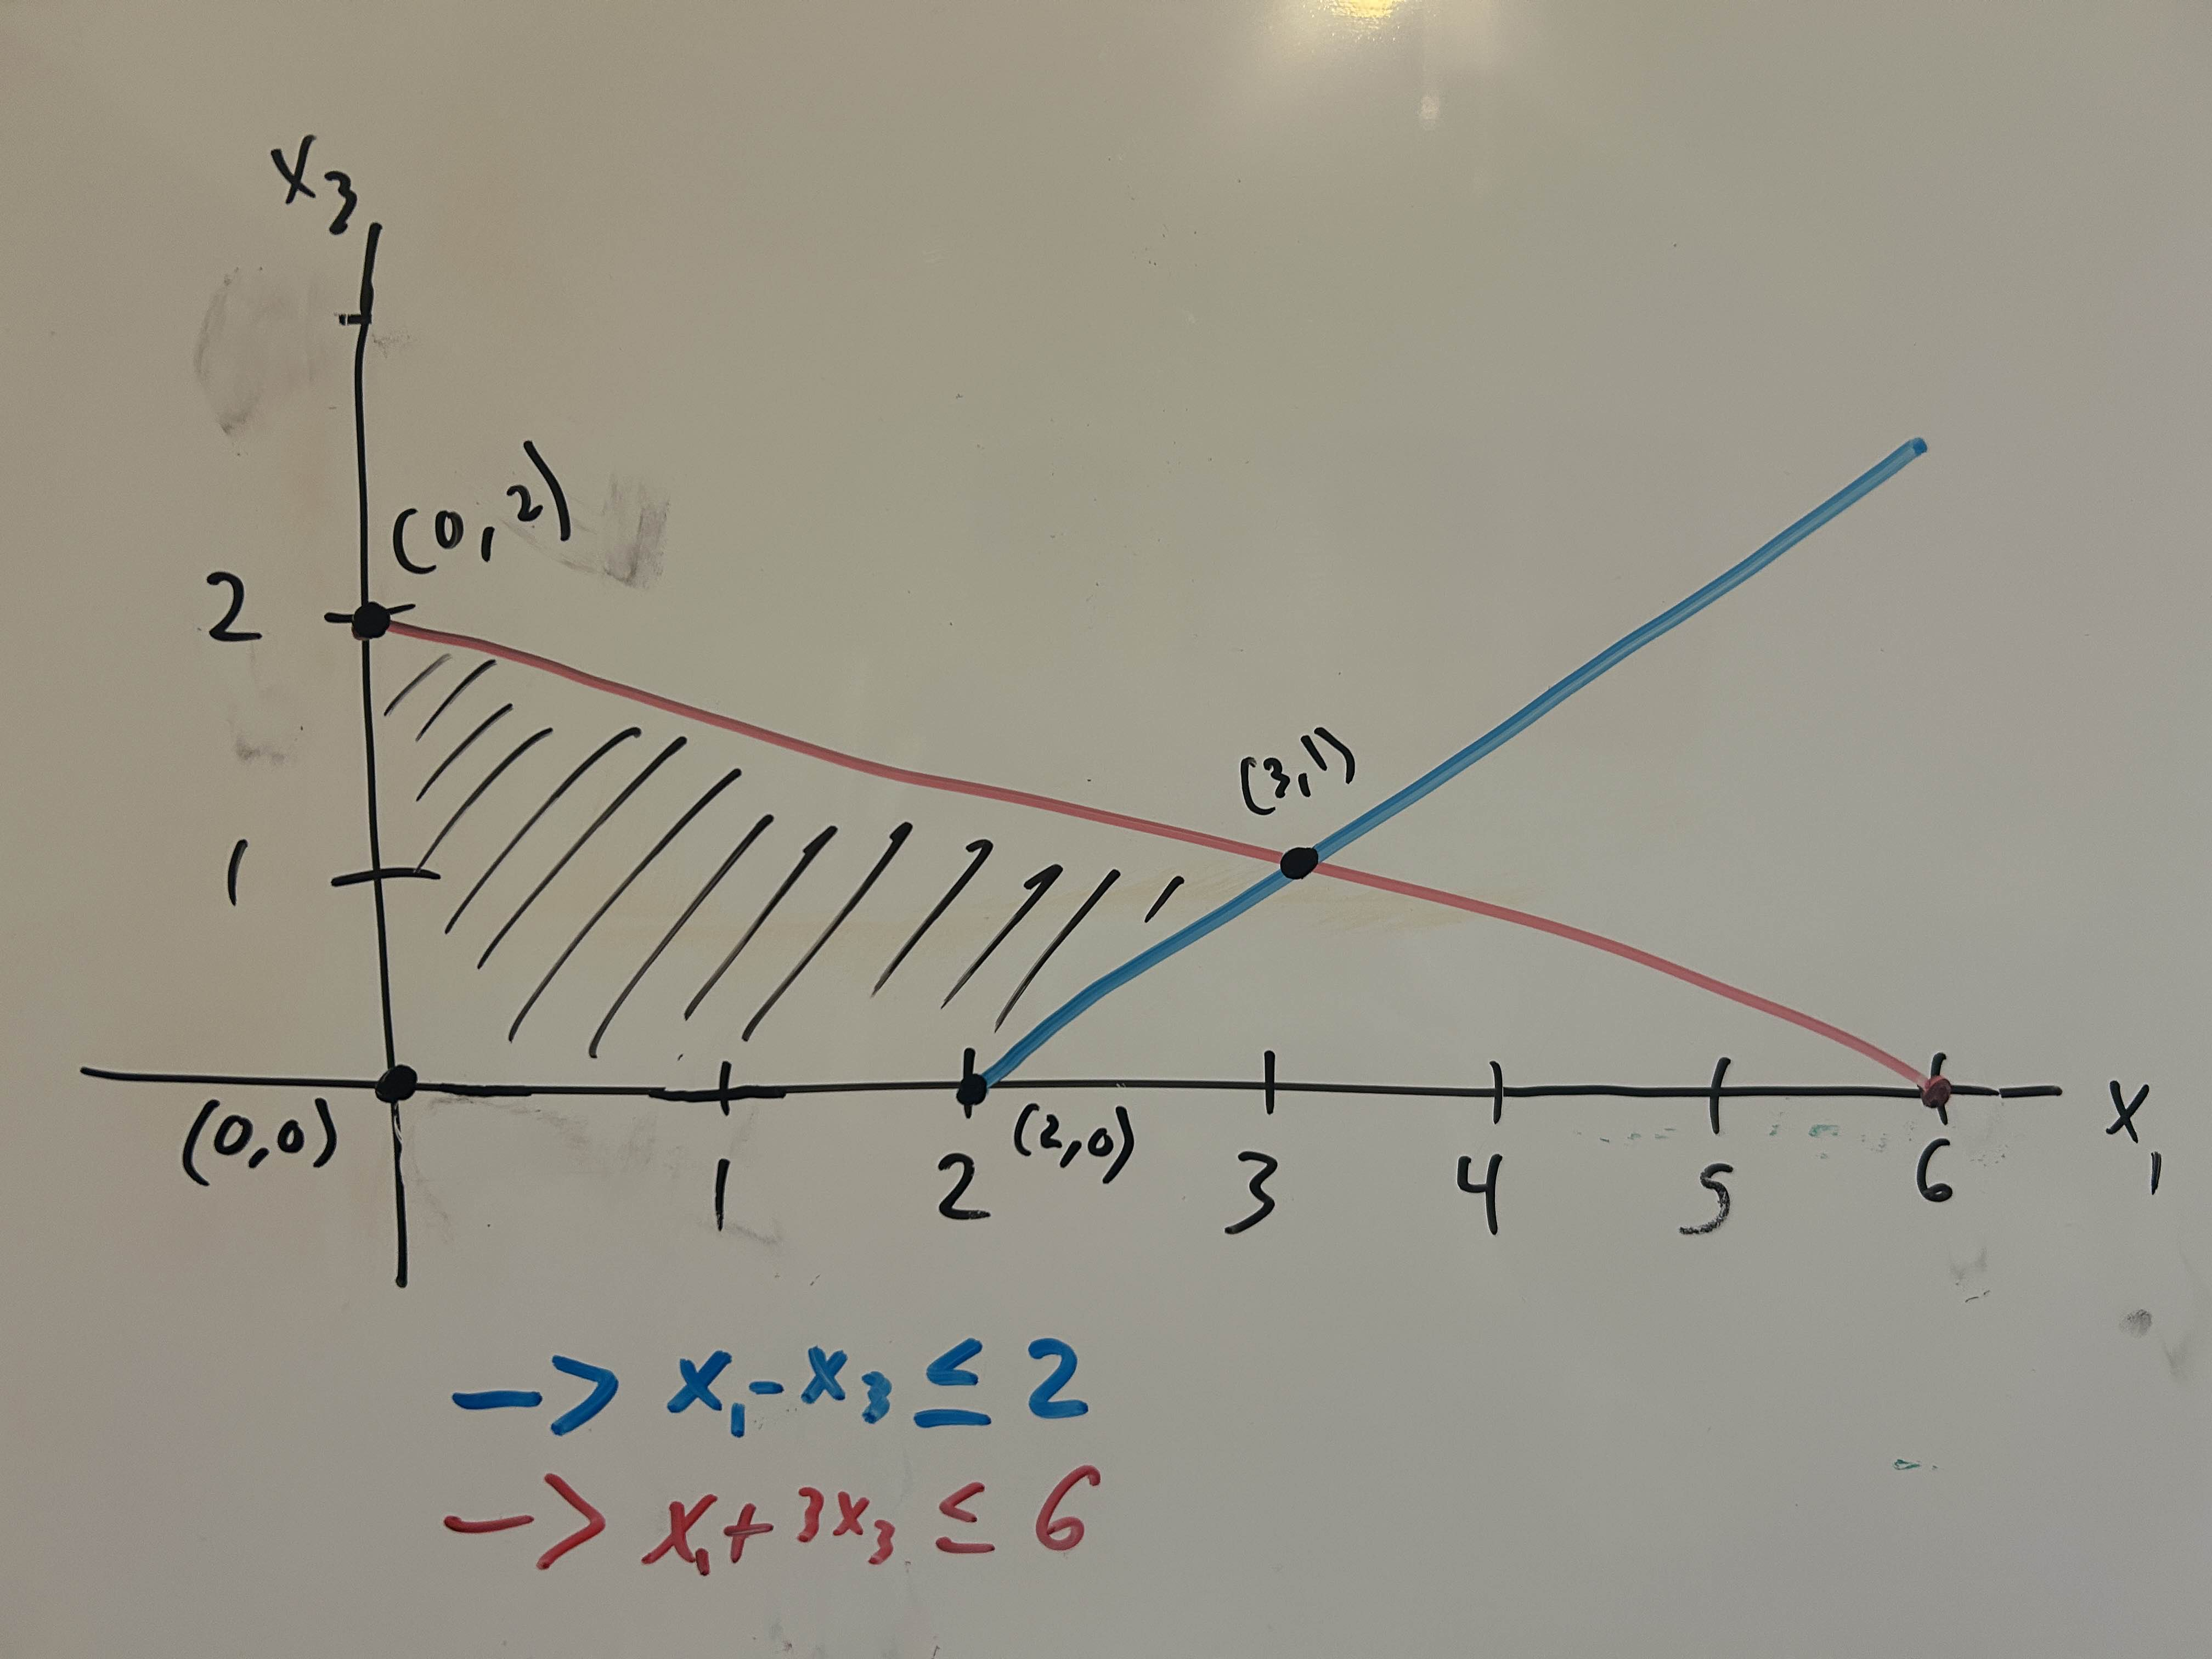
\includegraphics[width=0.8\textwidth]{../images/hw2.jpg}
    \caption{Feasible region of $x_1$ and $x_3$.}
    \label{fig:your_label}
\end{figure}